In this section, the layer is described in some detail in terms of its specific subsystems. Describe each of the layers and its subsystems in a separate chapter/major subsection of this document. The content of each subsystem description should be similar. Include in this section any special considerations and/or trade-offs considered for the approach you have chosen.

\subsection{Raspberry Pi}
In this system, the Raspberry Pi acts as the central hub that controls the traffic of data flow from one subsystem to another. It also activates functions of specific subsystems based on feedback from another subsystem.

\begin{figure}[h!]
	\centering
 	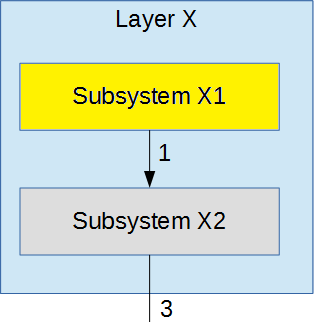
\includegraphics[width=0.60\textwidth]{images/subsystem}
 \caption{Example subsystem description diagram}
\end{figure}

\subsubsection{Assumptions}
The Raspberry Pi is assumed to be powered on throughout the active run time of the system. In addition to that, the Pi needs to have a persistent forms of connections with the other subsystems.

\subsubsection{Responsibilities}
Here is an overview of the data flow pathways that Pi is involved in:
\begin{itemize}
  \item After receiving a positive signal of drone detection from ODAS (which is in the Processing Subsystem), the Pi activates the secondary detector in the Detection Subsystem. 
  \item After receiving confirmation of drone detection from Secondary Processor, it relays relevant drone data to the Drone Algorithm Database.
  \item The Pi also has a bi-directional connection with I/O Subsystems, particularly with the Application subsystem. It is the point of contact in terms of setting updates and user-logins for the user of the system.
\end{itemize}

\subsubsection{Subsystem Interfaces}
Each of the inputs and outputs for the subsystem are defined here. Create a table with an entry for each labelled interface that connects to this subsystem. For each entry, describe any incoming and outgoing data elements will pass through this interface.

\begin {table}[H]
\caption {Subsystem interfaces} 
\begin{center}
    \begin{tabular}{ | p{1cm} | p{6cm} | p{3cm} | p{3cm} |}
    \hline
    ID & Description & Inputs & Outputs \\ \hline
    \#RP01 & Raspberry Pi & \pbox{3cm}{Signal from ODAS \\\hline Signal from secondary processor \\ \hline User inputs from Application} & \pbox{3cm}{Activation of secondary sensor in Detection subsystems \\\hline  Drone data relayed to Drone Algorithm Database \\\hline Feedback after processing user inputs back to Application}  \\ \hline
    \#RP02 & Raspberry Pi power & \pbox{3cm}{Power} & \pbox{3cm}{N/A}  \\ \hline
    \#RP03 & Raspberry Pi communications & \pbox{3cm}{Network, preferably wireless} & \pbox{3cm}{Connection pathways between subsystems established}  \\ \hline
    \end{tabular}
\end{center}
\end{table}

\subsection{Drone Algorithm Database}

\subsubsection{Assumptions}

\subsubsection{Responsibilities}

\subsubsection{Subsystem Interfaces}
\begin {table}[H]
\caption {Subsystem interfaces} 
\begin{center}
    \begin{tabular}{ | p{1cm} | p{6cm} | p{3cm} | p{3cm} |}
    \hline
    ID & Description & Inputs & Outputs \\ \hline
    \#xx & Description of the interface/bus & \pbox{3cm}{input 1 \\ input 2} & \pbox{3cm}{output 1}  \\ \hline
    \#xx & Description of the interface/bus & \pbox{3cm}{N/A} & \pbox{3cm}{output 1}  \\ \hline
    \end{tabular}
\end{center}
\end{table}

